% ------------------------------------------------------------------------------
% This figure is designed to be compiled separately as a standalone PDF.
% 
% For faster compilation of your main document:
% 1. Compile this .tex file independently to generate a PDF file.
% 2. Store the generated PDF (e.g., figure_demand.pdf) in your project's
%    'figures' folder (or another directory of your choice).
% 3. In your main document, include the figure PDF with:
%      \includegraphics{figures/figure_demand.pdf}
%
% This approach keeps the main document compilation fast and modular.
% ------------------------------------------------------------------------------

\documentclass[tikz]{standalone}

% Use sans-serif font for text and math
\renewcommand{\familydefault}{\sfdefault}
\usepackage{sfmath}

% Load pgfplots and set compatibility
\usepackage{pgfplots}
\pgfplotsset{compat=1.18}

% Load your custom color definitions
% TU Graz Colors
\definecolor{tug}{HTML}{F70146}

% IEE Color
\definecolor{iee}{HTML}{008080}
\colorlet{main}{iee}

% PowerPoint Palette
\definecolor{fore}{HTML}{0F0F0F}
\definecolor{back}{HTML}{FFFFFF}
\definecolor{dark}{HTML}{3B5A70}
\definecolor{lite}{HTML}{A6A6A6}
\definecolor{head}{HTML}{245B78}
\definecolor{body}{HTML}{E2E9ED}
\definecolor{urlA}{HTML}{0066D8}
\definecolor{urlB}{HTML}{6C2F91}
\colorlet{colA}{iee}
\colorlet{colB}{tug}
\definecolor{colC}{HTML}{6BA3A3}
\definecolor{colD}{HTML}{2E4172}
\definecolor{colE}{HTML}{78BE73}
\definecolor{colF}{HTML}{D58E00}
\colorlet{grey}{lite}
\colorlet{default}{dark}

% Alternate color names
\colorlet{blue}{dark}
\colorlet{turquoise}{colC}
\colorlet{green}{colE}
\colorlet{yellow}{colF}
\colorlet{red}{colB}

% Light Shades
\definecolor{greyLight}{HTML}{EDEDED}
\definecolor{blueLight}{HTML}{D3DFE8}
\definecolor{ieeLight}{HTML}{E1EDED}
\definecolor{redLight}{HTML}{FFCBDA}
\definecolor{turquoiseLight}{HTML}{E1EDED}
\definecolor{greenLight}{HTML}{E4F2E3}
\definecolor{yellowLight}{HTML}{FFEBC4}

% Dark Shades
\definecolor{greyDark}{HTML}{0F0F0F}
\definecolor{blueDark}{HTML}{1D2D38}
\definecolor{ieeDark}{HTML}{004040}
\definecolor{redDark}{HTML}{7C0023}
\definecolor{turquoiseDark}{HTML}{345353}
\definecolor{greenDark}{HTML}{346830}
\definecolor{yellowDark}{HTML}{6A4700}

% Power Plant Colors
\definecolor{oilColor}{RGB}{16, 47, 64}
\definecolor{coalColor}{RGB}{127, 127, 127}
\definecolor{gasColor}{RGB}{191, 191, 191}
\definecolor{otherNonResColor}{RGB}{221, 110, 56}
\definecolor{nuclearColor}{RGB}{236, 96, 95}
\definecolor{biomassColor}{RGB}{198, 70, 59}
\definecolor{rorColor}{RGB}{0, 176, 240}
\definecolor{pvColor}{RGB}{255, 192, 0}
\definecolor{windColor}{RGB}{146, 208, 80}
\definecolor{windOffColor}{RGB}{30, 143, 79}
\definecolor{otherResColor}{RGB}{185, 207, 222}
\definecolor{storageHydroColor}{RGB}{75, 172, 198}
\definecolor{pumpedStorageColor}{RGB}{59, 90, 112}
\definecolor{bessColor}{RGB}{112, 48, 160}
\definecolor{otherStorageColor}{RGB}{76, 133, 123}

\begin{document}
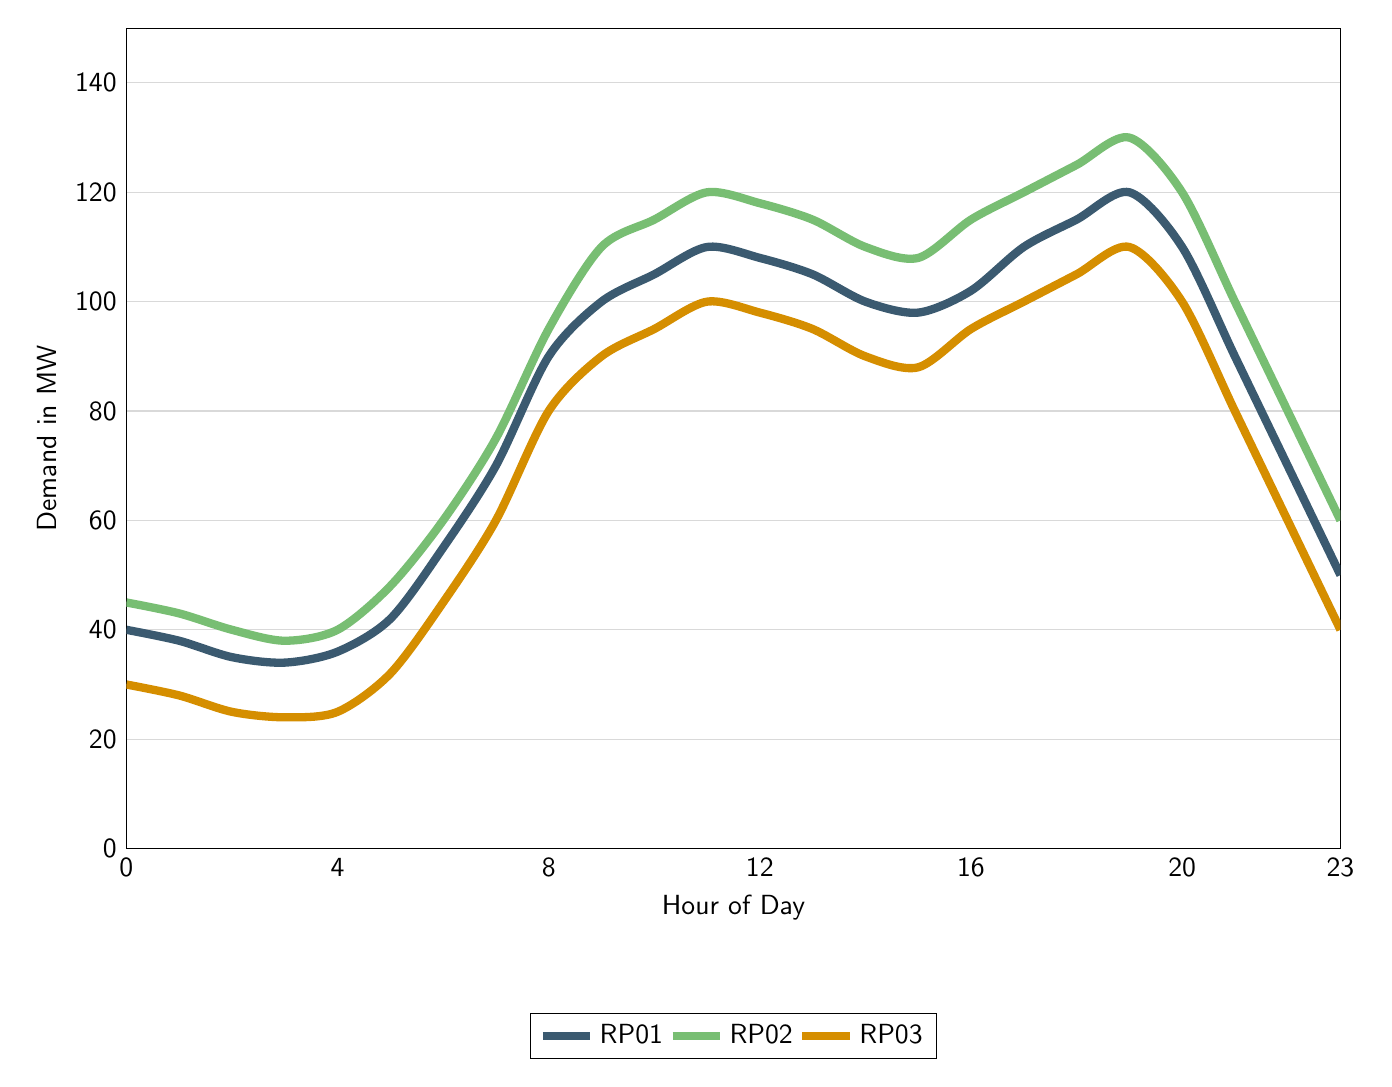
\begin{tikzpicture}
    \begin{axis}[
        width=17cm,
        height=12cm,
        xlabel={Hour of Day},
        ylabel={Demand in MW},
        xmin=0, xmax=23,
        ymin=0, ymax=150,
        xtick={0,4,8,12,16,20,23},
        ymajorgrids=true,
        grid style={gray!30},
        legend style={at={(0.5,-0.2)}, anchor=north, legend columns=3},
        tick style={draw=none},
        axis line style={black},
        legend cell align={left},
        tick label style={font=\sffamily},
    ]

    % Sample data for Day 1
    \addplot+[mark=none, line width=3pt, smooth, color=default] coordinates {
        (0,40) (1,38) (2,35) (3,34) (4,36) (5,42)
        (6,55) (7,70) (8,90) (9,100) (10,105) (11,110)
        (12,108) (13,105) (14,100) (15,98) (16,102) (17,110)
        (18,115) (19,120) (20,110) (21,90) (22,70) (23,50)
    };

    % Sample data for Day 2
    \addplot+[mark=none, line width=3pt, smooth, color=green] coordinates {
        (0,45) (1,43) (2,40) (3,38) (4,40) (5,48)
        (6,60) (7,75) (8,95) (9,110) (10,115) (11,120)
        (12,118) (13,115) (14,110) (15,108) (16,115) (17,120)
        (18,125) (19,130) (20,120) (21,100) (22,80) (23,60)
    };

    % Sample data for Day 3
    \addplot+[mark=none, line width=3pt, smooth, color=yellow] coordinates {
        (0,30) (1,28) (2,25) (3,24) (4,25) (5,32)
        (6,45) (7,60) (8,80) (9,90) (10,95) (11,100)
        (12,98) (13,95) (14,90) (15,88) (16,95) (17,100)
        (18,105) (19,110) (20,100) (21,80) (22,60) (23,40)
    };

    \legend{RP01, RP02, RP03}
    \end{axis}
\end{tikzpicture}
\end{document}